\documentclass[tikz,border=12pt]{standalone}
% Shared visual language for standalone EMT block diagrams.
\usepackage{amsmath}
\usetikzlibrary{arrows.meta,backgrounds,calc,fit,positioning}

\tikzset{
    emt diagram/.style = {>={Stealth[length=2.4mm]}},
    line/.style        = {semithick, rounded corners=6pt},
    block/.style       = {draw, semithick, fill=white,
                          minimum height=1cm, minimum width=2.3cm},
    hblock/.style      = {block, minimum width=2.24cm, minimum height=1.3cm},
    vblock/.style      = {block, minimum width=1.3cm, minimum height=2.24cm},
    sum/.style         = {draw, semithick, fill=white, circle,
                          inner sep=2.6pt},
    signal/.style      = {circle, fill, inner sep=1.4pt,
                          label distance=3pt},
    sig/.style         = {font=\small},
    pm/.style          = {font=\scriptsize},
    wire jump/.style   = {line,
                          preaction={draw=white, line width=3pt,
                                     line cap=round}},
    enclosure/.style   = {draw, dashed, semithick, rounded corners=4pt},
    operator enclosure/.style = {enclosure, inner xsep=7mm, inner ysep=6mm}
}


% TUNABLES: gain width and spacing of the two lower branches.
\def\gainwidth{1.35cm}
\def\integralrow{-1.9}
\def\trackingrow{-3.8}

\begin{document}
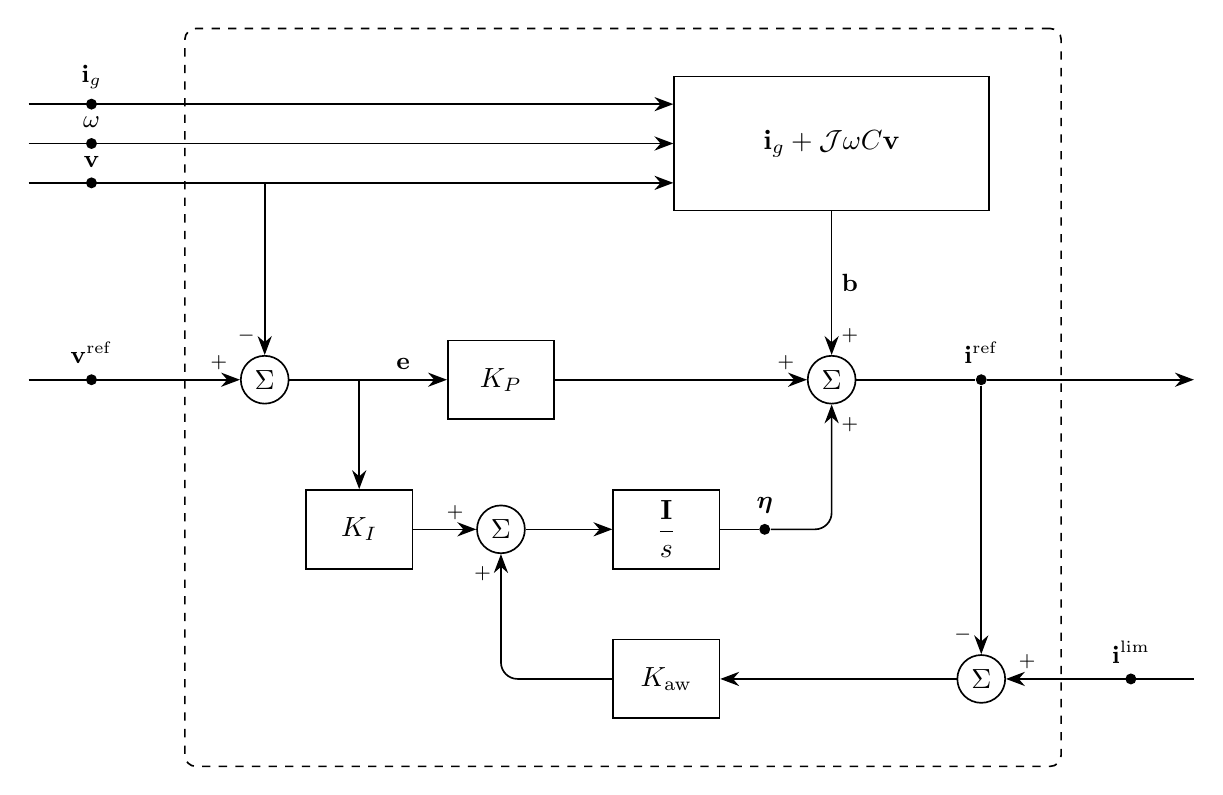
\begin{tikzpicture}[emt diagram]

% Voltage error and proportional path.
\node[sum] (error) at (0,0) {$\Sigma$};
\coordinate (esplit) at (1.2,0);
\node[block, minimum width=\gainwidth] (Kp) at (3,0) {$K_P$};
\node[sum] (command) at (7.2,0) {$\Sigma$};
\draw[line] (error.east) -- (esplit);
\draw[->, line] (esplit) -- node[sig, above] {$\mathbf{e}$} (Kp.west);
\draw[->, line] (Kp.east) -- (command.west);
\node[pm, above left=0pt and 1pt of command.west] {$+$};

% Integral path, with anti-windup added before integration.
\node[block, minimum width=\gainwidth] (Ki)
    at (1.2,\integralrow) {$K_I$};
\node[sum] (rate) at (3,\integralrow) {$\Sigma$};
\node[block, minimum width=\gainwidth] (integrator)
    at (5.1,\integralrow) {$\dfrac{\mathbf{I}}{s}$};
\node[signal, label={[sig]above:$\boldsymbol{\eta}$}] (eta)
    at (6.35,\integralrow) {};
\draw[->, line] (esplit) -- (Ki.north);
\draw[->, line] (Ki.east) -- (rate.west);
\node[pm, above left=0pt and 1pt of rate.west] {$+$};
\draw[->, line] (rate.east) -- (integrator.west);
\draw[line] (integrator.east) -- (eta);
\draw[->, line] (eta) -| (command.south);
\node[pm, below right=1pt and 0pt of command.south] {$+$};

% Grid-current feedforward and capacitor-current decoupling.
\node[block, minimum width=4cm, minimum height=1.7cm]
    (feedforward) at (7.2,3)
    {$\mathbf{i}_g+\mathcal{J}\omega C\mathbf{v}$};
\draw[->, line] (feedforward.south)
    -- node[sig, right] {$\mathbf{b}$} (command.north);
\node[pm, above right=1pt and 0pt of command.north] {$+$};

% Total current reference supplied to the inner current controller.
\node[signal, label={[sig]above:$\mathbf{i}^{\mathrm{ref}}$}]
    (iref) at (9.1,0) {};
\draw[line] (command.east) -- (iref);
\draw[->, line] (iref) -- (11.8,0);

% Track the current limit owned by the inner current controller.
\node[sum] (tracking) at (9.1,\trackingrow) {$\Sigma$};
\node[block, minimum width=\gainwidth] (Kaw)
    at (5.1,\trackingrow) {$K_{\mathrm{aw}}$};
\draw[->, line] (iref) -- (tracking.north);
\node[pm, above left=1pt and 0pt of tracking.north] {$-$};
\draw[->, line] (tracking.west) -- (Kaw.east);
\draw[->, line] (Kaw.west) -| (rate.south);
\node[pm, below left=1pt and 0pt of rate.south] {$+$};

% External inputs share the same frame and signal ownership conventions.
\node[signal, label={[sig]above:$\mathbf{v}^{\mathrm{ref}}$}]
    (vref) at (-2.2,0) {};
\node[signal, label={[sig]above:$\mathbf{v}$}] (v) at (-2.2,2.5) {};
\node[signal, label={[sig]above:$\omega$}] (omega) at (-2.2,3) {};
\node[signal, label={[sig]above:$\mathbf{i}_g$}] (ig) at (-2.2,3.5) {};
\node[signal, label={[sig]above:$\mathbf{i}^{\mathrm{lim}}$}]
    (ilim) at (11,\trackingrow) {};
\coordinate (vsplit) at (error |- v);
\draw[->, line] ($(vref)+(-0.8,0)$) -- (error.west);
\node[pm, above left=0pt and 1pt of error.west] {$+$};
\draw[->, line] ($(v)+(-0.8,0)$) -- (feedforward.west |- v);
\draw[->, line] (vsplit) -- (error.north);
\node[pm, above left=1pt and 0pt of error.north] {$-$};
\draw[->, line] ($(omega)+(-0.8,0)$) -- (feedforward.west |- omega);
\draw[->, line] ($(ig)+(-0.8,0)$) -- (feedforward.west |- ig);
\draw[->, line] ($(ilim)+(0.8,0)$) -- (tracking.east);
\node[pm, above right=0pt and 1pt of tracking.east] {$+$};

% Enclose the model-owned states, variables, and feedback paths.
\begin{scope}[on background layer]
    \node[operator enclosure,
        fit=(error)(Kp)(Ki)(rate)(integrator)(eta)
            (feedforward)(command)(iref)(tracking)(Kaw)] {};
\end{scope}

\end{tikzpicture}
\end{document}
